% **************************** Define Graphics Path **************************
\ifpdf
\graphicspath{{Chapter3/Figs/Raster/}{Chapter3/Figs/PDF/}{Chapter3/Figs/}{Chapter3/Figs/Web/}{Chapter3/Figs/Server/}{Chapter3/Figs/Mobile/}}
\else
\graphicspath{{Chapter3/Figs/Vector/}{Chapter3/Figs/}}
\fi

\chapter{Thiết kế và Hiện thực}

\section{Thiết kế hệ thống}
\subsection{Kiến trúc mô hình hệ thống}


Lorem ipsum dolor sit amet, consectetur adipiscing elit, sed do eiusmod tempor incididunt ut labore et dolore magna aliqua. Ut enim ad minim veniam, quis nostrud exercitation ullamco laboris nisi ut aliquip ex ea commodo consequat. Duis aute irure dolor in reprehenderit in voluptate velit esse cillum dolore eu fugiat nulla pariatur. Excepteur sint occaecat cupidatat non proident, sunt in culpa qui officia deserunt mollit anim id est laborum
\subsubsection*{Cách thức tương tác cập nhật dữ liệu}

Trong việc tương tác cập nhật dữ liệu, hiện nay mô hình truy thường được sử dụng là \textbf{polling}. Client và server phải liên tục gửi các request liên tục cách nhau trong một thời gian cố định để kiểm tra liệu có sự thay đổi cập nhật dữ liệu. 
\begin{figure}[H]
	\centering    
	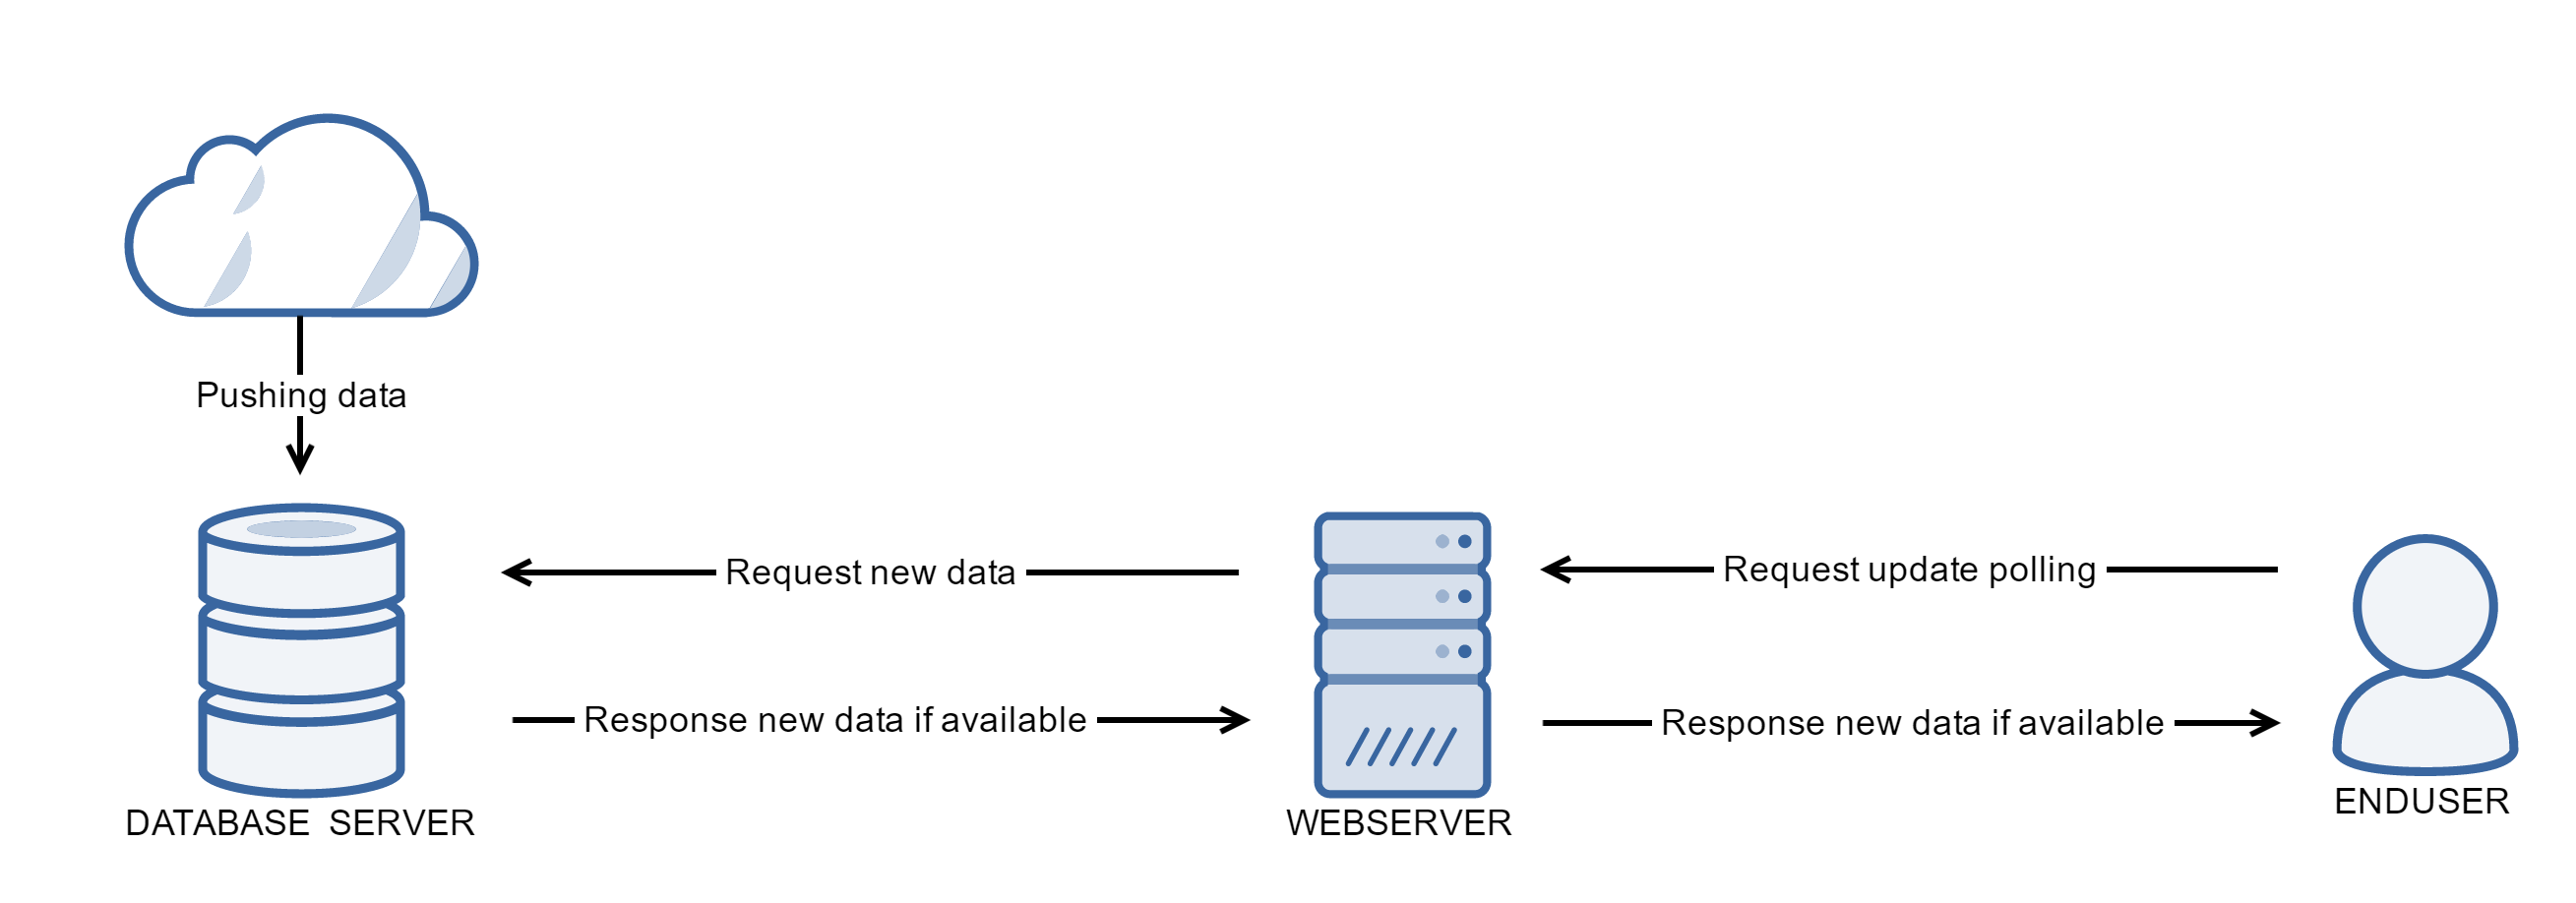
\includegraphics[width=1.0\textwidth]{polling}
	\caption[Mô hình tương tác polling]{Mô hình tương tác polling}
	\label{fig: polling}
\end{figure}
Phương pháp này dễ hiện thực và áp dụng, tuy nhiên sẽ mắc nhược điểm là tốn nhiều gói tin request vô dụng làm giảm hiệu năng hệ thống, và không đáp ứng tính realtime nếu như chu kì gửi request dài.



Vì hiện tại nhóm chúng tôi đang hướng tới hướng phát triển IoT, đòi hỏi yêu cầu về tính realtime cũng như tối ưu hóa hệ thống. Và để đáp ứng yêu cầu đó, nhóm đã tìm tới giải pháp giữ socket kết nối từ \textbf{Database} (RethinkDB) <-> \textbf{Server} (Chạy trên nền tảng Nodejs) <-> \textbf{Client} (web browser)

\begin{figure}[H]
	\centering    
	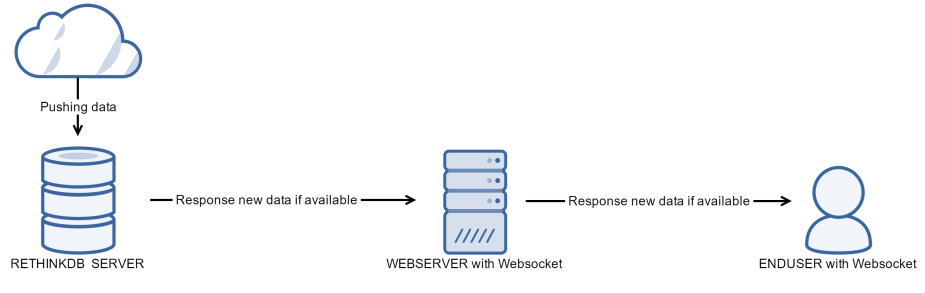
\includegraphics[width=1.0\textwidth]{realtime}
	\caption[Mô hình tương tác realtime dựa trên Socket]{Mô hình tương tác realtime dựa trên Socket}
	\label{fig: realtime}
\end{figure}

Như hình \ref{fig: realtime}, mô hình hoạt động đơn giản hơn rất nhiều, giảm bớt số lượng request không đáng có và đảm bảo tính realtime cho hệ thống.

Một điểm mạnh ở mô hình này nữa là có thể phát triển nhiều server hoặc ứng dụng di động sử dụng chung một hệ quản lý cơ sở dữ liệu nhưng vẫn đảm bảo sự đồng bộ dữ liệu cập nhật tới enduser theo thời gian thực.
\begin{figure}[H]
	\centering    
	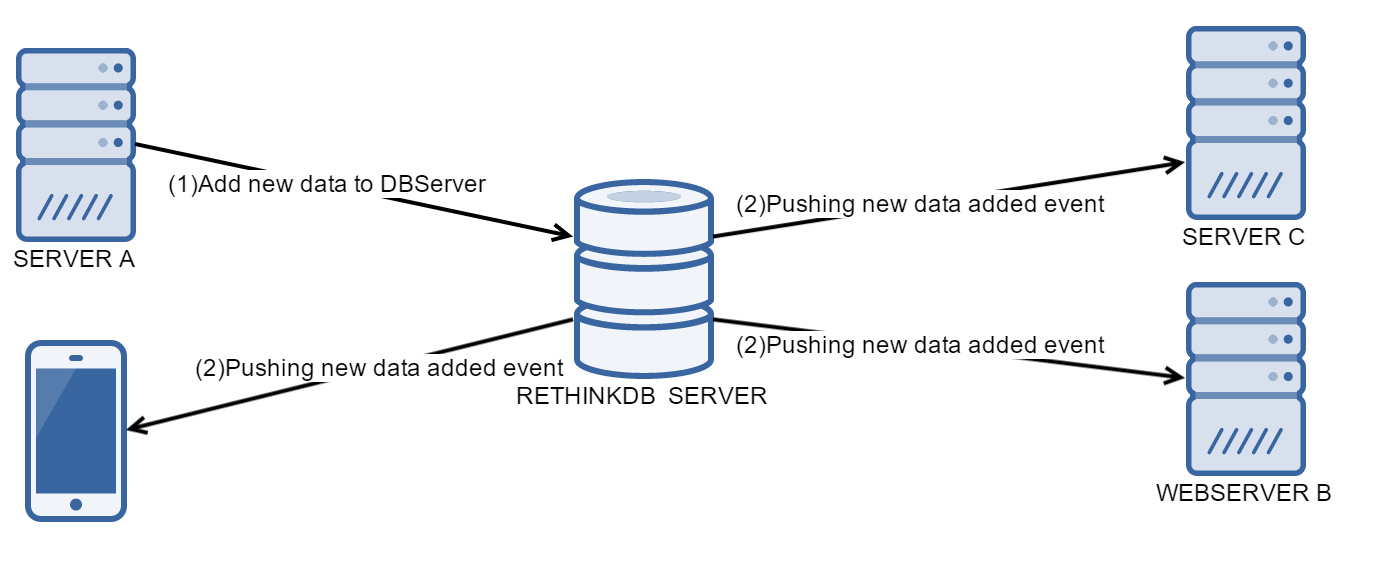
\includegraphics[width=1.0\textwidth]{multiserver}
	\caption[Mô hình tương tác cập nhật nhiều Server]{Mô hình tương tác cập nhật nhiều Server}
	\label{fig: multiserver}
\end{figure}
\subsection{Các ràng buộc của hệ thống}
Lorem ipsum dolor sit amet, consectetur adipiscing elit, sed do eiusmod tempor incididunt ut labore et dolore magna aliqua. Ut enim ad minim veniam, quis nostrud exercitation ullamco laboris nisi ut aliquip ex ea commodo consequat. Duis aute irure dolor in reprehenderit in voluptate velit esse cillum dolore eu fugiat nulla pariatur. Excepteur sint occaecat cupidatat non proident, sunt in culpa qui officia deserunt mollit anim id est laborum
\subsection{Mô hình ứng dụng trình bày dữ liệu}
Lorem ipsum dolor sit amet, consectetur adipiscing elit, sed do eiusmod tempor incididunt ut labore et dolore magna aliqua. Ut enim ad minim veniam, quis nostrud exercitation ullamco laboris nisi ut aliquip ex ea commodo consequat. Duis aute irure dolor in reprehenderit in voluptate velit esse cillum dolore eu fugiat nulla pariatur. Excepteur sint occaecat cupidatat non proident, sunt in culpa qui officia deserunt mollit anim id est laborum
\section{Hiện thực Node cảm biến}
\subsection{Các node cảm biến thu thập dữ liệu}
Lorem ipsum dolor sit amet, consectetur adipiscing elit, sed do eiusmod tempor incididunt ut labore et dolore magna aliqua. Ut enim ad minim veniam, quis nostrud exercitation ullamco laboris nisi ut aliquip ex ea commodo consequat. Duis aute irure dolor in reprehenderit in voluptate velit esse cillum dolore eu fugiat nulla pariatur. Excepteur sint occaecat cupidatat non proident, sunt in culpa qui officia deserunt mollit anim id est laborum
\subsection{Ứng dụng theo dõi dữ liệu và đánh giá}
Lorem ipsum dolor sit amet, consectetur adipiscing elit, sed do eiusmod tempor incididunt ut labore et dolore magna aliqua. Ut enim ad minim veniam, quis nostrud exercitation ullamco laboris nisi ut aliquip ex ea commodo consequat. Duis aute irure dolor in reprehenderit in voluptate velit esse cillum dolore eu fugiat nulla pariatur. Excepteur sint occaecat cupidatat non proident, sunt in culpa qui officia deserunt mollit anim id est laborum
\section{Hệ thống Server lưu trữ dữ liệu và cung cấp API}
Lorem ipsum dolor sit amet, consectetur adipiscing elit, sed do eiusmod tempor incididunt ut labore et dolore magna aliqua. Ut enim ad minim veniam, quis nostrud exercitation ullamco laboris nisi ut aliquip ex ea commodo consequat. Duis aute irure dolor in reprehenderit in voluptate velit esse cillum dolore eu fugiat nulla pariatur. Excepteur sint occaecat cupidatat non proident, sunt in culpa qui officia deserunt mollit anim id est laborum
\subsection{Cấu trúc tổ chức tập tin}
\subsubsection*{Các thư mục và chức năng}
\begin{figure}[H]
	\centering    
	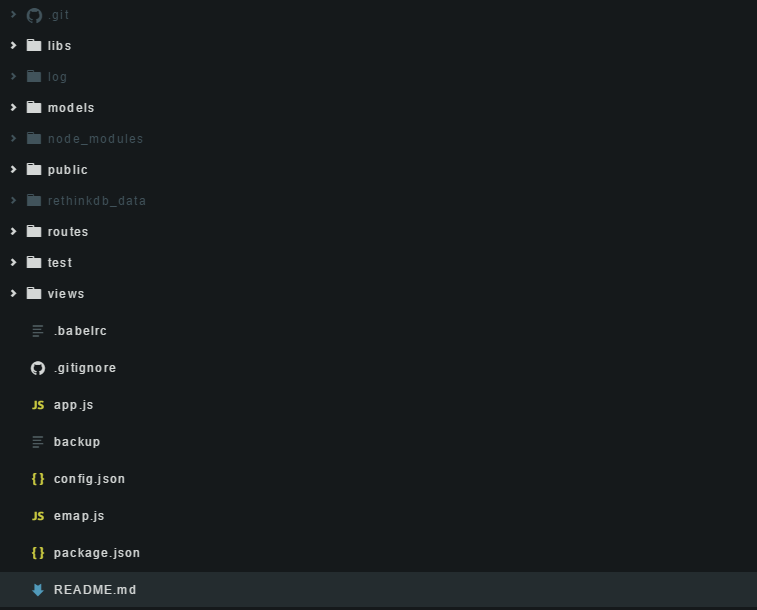
\includegraphics[width=1.0\textwidth]{tree}
	\caption[Mô hình hoạt động Nodejs]{Mô hình hoạt động Nodejs}
	\label{fig: tree}
\end{figure}
Như hình \ref{fig: tree}, chúng ta có những thư mục được làm việc trực tiếp:

• libs: chứa các hàm function hỗ trợ về xác thực và log.

• models: thư mục này bao gồm các mô hình quản lý cơ sở dữ liệu.

• routes: điều khiển và điều hướng theo các url.

• log: chứa các file ghi lại log trong quá trình hoạt động.

• views: là bộ mặt của web server, giúp người dùng có thể tương tác được với server qua web browser, bao gồm các file giao diện như html, ejs...   


\subsubsection*{Các file khởi tạo và cấu hình Server}

\textbf{Các file khởi tạo này bao gồm:}

• emap.js: file có chức năng đọc file cấu hình và khởi tạo kết nối server.
\begin{lstlisting}[caption=emap.js]
...
server.on('listening', onListening); // open for listening
function onListening() {
	var addr = server.address();
	var bind = typeof addr === 'string' ?
	'pipe' + addr :
	'port' + addr.port;
	debug('Listening on ' + bind);
	console.log('Listening on ' + bind);
};
...
\end{lstlisting}

• app.js: là file điều khiển và thiết lập các chức năng, khai báo các modules chính được sử dụng. Bên cạnh đó, còn có chức năng gán điều hướng tới các file trong thư mục route
\begin{lstlisting}[caption=app.js]
...
// initial server
app.use(passport.initialize());
app.use(passport.session());
app.set('views', path.join(\_\_dirname, 'views'));
app.engine('ejs', engine);
...
// control route
app.use(logger('dev'));
app.use('/log', express.static(path.join(__dirname, 'log')));
app.use(express.static(path.join(__dirname, 'public')));
app.use('/log', serveIndex('./log'));
app.use('/', routes);
app.use('/user', user);
app.use('/node', node);
app.use('/auth', auth);
...
\end{lstlisting}

\textbf{Các file cấu hình này bao gồm:}

• package.json: khai báo các thông tin cơ bản về project và các modules được sử dụng.
\begin{lstlisting}[caption=package.json]
{
	"name": "emap-server",
	"version": "1.0.0",
	"description": "This is serverside part of IoT project",
	"main": "emap.js",
	"author": "Cuong, Tung and Ny",
	"license": "ISC",
	"homepage": "www.codingyourfuture.com",
	"dependencies": {			// dependancies modules
		"angular-chart.js": "^1.0.3",
		"asyncawait": "^1.0.6",
		"babel": "^6.5.2",
		"ejs": "^2.5.2",
		...
		"rethinkdb": "^2.3.3",
		"serve-index": "^1.8.0",
		"socket.io": "^1.5.0",
	}
}
\end{lstlisting}
• config.json: khai báo các thông số cấu hình được sử dụng. Tại đây ta cấu hình thông số kết nối tới RethinkDB và port ứng dụng server nodejs.
\begin{lstlisting}[caption=config.json]
{
	"app":{
		"port": "8888"
	},
	"rethinkdb":{
		"host": "localhost",
		"port" : "28015",
		"db": "emap",
		"address":"localhost:28015",
		"tableList":["nodeData"]
	}
}

\end{lstlisting}


%% Thiết kế API

\subsection{Thiết kế API}

Mục tiêu đề tài không chỉ thu thập và phân tích mà còn chia sẻ dữ liệu. Để làm được điều đó thì cần phải có API cung cấp cho những nhà phát triển thứ 3, có thể dùng API được cung cấp để sử dụng dữ liệu để phát triển. Bởi vì vậy hệ thống có xây dựng hệ thống API mở.

\subsubsection*{API List}
Ở bảng \ref{table: apilist}
\begin{table}[H]
	\centering
	\caption{Bảng API tương tác với dữ liệu về các node}
	\begin{tabular}{|l|l|l|l|}
		\hline
		Method & URL            & Miêu tả         & Yêu cầu xác thực người dùng        \\ \hline
		POST   & /node/initnew       & Khởi tạo node mới                & Có           \\ \hline
		POST   & /node/updatenode     & Cập nhật thông tin node & Có \\ \hline
		POST   & /node/replacenode       & Thay thế node  & Có       \\ \hline
		GET   & /node/pushdata & Push dữ liệu               &         Không                \\ \hline
		GET   & /node/getdata    & Get dữ liệu thu thập của node         &  Không      \\ \hline
		GET   & /node/getinfo   & Get thông tin của node & Không  \\ \hline
	\end{tabular}
	\label{table: apilist}
\end{table}

/node/initnew
/node/pushdata
/node/updatenode
/node/replacenode
/node/getdata
/node/getinfo



\subsection{Hiện thực Server}
\subsection{Xây dựng Web Server}
\subsection*{Chức năng}

\subsubsection*{Đối với người dùng:}
Hiện thị các node cảm biến đang hoạt động trên google map, cung cấp các thông tin liên quan đến node( vị trí địa lí, tình trạng hoạt động, biểu đồ theo thời gian thực của các dữ liệu mà node thu thập được), giao tiếp với người quản lý thông qua gmail.
\subsubsection*{Đối với người quản trị:}
Bao gồm các chức năng tương tự như người dùng và thêm việc quản lý chỉnh sửa thông tin của các node: thêm, xóa, cập nhật, thay đổi…

\subsection*{Biểu đồ High level Usecase }

\begin{center}
\begin{figure}[htp]
\centering    
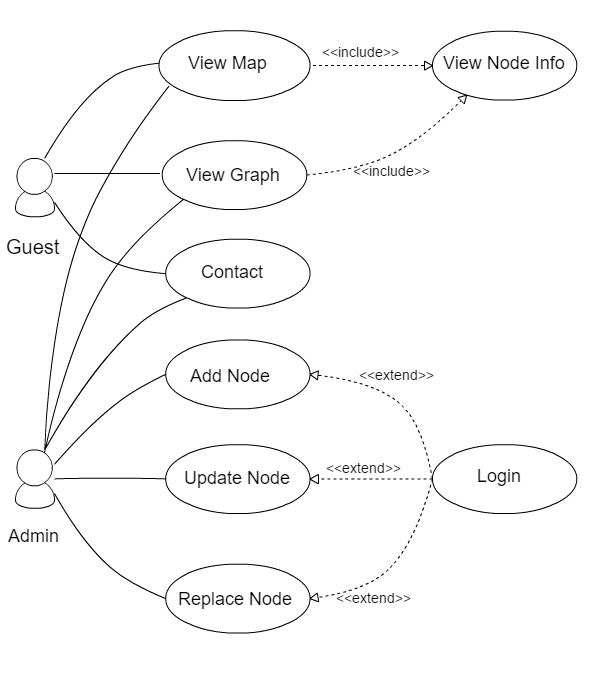
\includegraphics[width=0.7\textwidth]{usecase_diagram}
\caption[Biểu đồ High level Usecase]{Biểu đồ High level Usecase }
\label{fig:usecase_diagram}
\end{figure}
\end{center}

Mô tả giản đồ Usecase

\begin{table}[]
\centering
\caption{Bảng mô tả giản đồ Usecase}
\label{my-label}
\begin{tabular}{|l|l|l|}
\hline
STT & Tên            & Miêu tả                                                                                            \\ \hline
1   & View map       & Người dùng thấy được các node đang chạy trên google maps                                           \\ \hline
2   & View Node Info & Thông tin tương ứng của Node( Lat, Lng, Phone)                                                     \\ \hline
3   & View Graph     & \begin{tabular}[c]{@{}l@{}}Đồ thị hoạt động của Node(các số liệu đo được theo\\ ngày)\end{tabular} \\ \hline
4   & Contact        & Phản hồi ý kiến người dùng qua Gmail                                                               \\ \hline
5   & Add Node       & Thêm mới Node vào hoạt động                                                                        \\ \hline
6   & Update Node    & Thay đổi thông tin của Node( Lat, Lng, Phone)                                                      \\ \hline
7   & Replace Node   & Thay đổi 1 Node xảy ra sự cố bằng 1 Node khác                                                      \\ \hline
\end{tabular}
\end{table}





\subsection*{Hiện thực giao diện}

\subsection*{Sử dụng framework express của Nodejs và HTML để xây dựng frontend.}




-	Phần này chứa các nút menu chức năng cùng với google map để theo dõi vị trí hoạt động của các cảm biến




-	Là nơi hiện thị biểu đồ của các thông số cũng như thông tin tương ứng của các cảm biến.


-	Tương tác giữa người dùng với người quản lý server. Nội dung được gửi thông qua gmail.



-	Đăng nhập quản lý trang của admin( cho phép add, remove, replace, config các node cảm biến)



-	Hiện thị bảng tin(Cho phép thực hiện các chức năng chỉnh sửa trực tiếp trên map) cũng như tên người dùng sau khi đăng nhập.














\section{Ứng dụng thiết bị di động}

\subsection*{Chức năng}
Hiện thị thông tin các node đang hoạt động qua màn hình chính, kết nối với web browser tạo sự thuận tiện cho việc theo dõi, hiện thị đồ thị(2 kiểu đồ thị là line chart và bar chart).

\subsection*{Biểu đồ High level Usecase }
